\documentclass[10pt,journal,compsoc]{IEEEtran} \ifCLASSOPTIONcompsoc
 \usepackage[nocompress]{cite}
 \else
  \usepackage{cite} \fi
 \usepackage[latin1]{inputenc}
 \usepackage[T1]{fontenc}
 \usepackage{amsmath}
 \usepackage{amsfonts}
 \usepackage{amssymb}
 \usepackage{makeidx}
 \usepackage{graphicx}
 \usepackage{float}
 \usepackage{ifpdf}
 \ifpdf
 \usepackage[breaklinks,hidelinks]{hyperref}
 \else 
 \usepackage{url}
 \fi
 \begin{document} 
 \title{An Introduction to Process Variability Simulation} \author{Celso Bation Co \\ 
 Research and Development Office\\ Technological Institute of the Philippines\\ Quezon City, Philippines\\ celso.co@tip.edu.ph\\ \ 
 \IEEEcompsocitemizethanks{\IEEEcompsocthanksitem Technological Institute of the Philippines
} \thanks{Manuscript received March 18, 2019}}
 \maketitle
 \markboth{$29^{th}$ ASEMEP National Technical Symposium}%
    {Shell \MakeLowercase{	extit{et al.}}: Bare Advanced Demo of     IEEEtran.cls for IEEE Computer Society Journals}\noindent \begin{abstract}The processs variability covers typically the material, equipment, method,  and man, the so-called 4 Ms'.  A simple process of cutting a 10-meter rod into  two equal halves is illustrated where all the 4Ms were treated. The simulation  of variability for the 4 Ms' were discussed. The theoretical perspective  has caveat on matter of mathematical expressions that are realistics. The  algorith used was Monte Carlo Simulation based on random number generation that  fit Gaussian Curve. The python programming language was used with symbolic  math library, the sympy. Although the industry is used to 99.99\%, for the  sake tutotial the academe toys around 50\%. \end{abstract}
\noindent \begin{IEEEkeywords}variability, Normal Distribution, Gausian, Man, Machine, Method, Material,     4Ms.\end{IEEEkeywords}
\noindent \section{Introduction}
\noindent The Monte Carlo Simulation requires the generation of random variable of     which statistical distribution follows a certain distribution.  In this     case, the normal or Gaussian distribution is used based on the assertion that a     stable process must obey central tendency theorem. \\ \\     The Gaussian distribution function\cite{20} is stated as follows.
\begin{equation}
\begin{minipage}{300pt}
 $\displaystyle f(x) = \frac{\sqrt{2} e^{- \frac{\left(\mu - x\right)^{2}}{2 \sigma^{2}}}}{2 \sqrt{\pi} \sigma}$  
\end{minipage}
\end{equation}
\noindent where :	\\ $\mu$    : Real number or a list representing the mean or the mean vector \\ $\sigma$ : Real number or a positive definite square matrix, \\ $\sigma^{2} > 0 $ the variance \\ Returns: A Random Symbol. \\ \\ 
\noindent The sympy function 
\begin{equation}
\begin{minipage}{300pt}
 $\displaystyle f_{1} = NormalDistribution(\mu, \sigma)$  
\end{minipage}
\end{equation}
\noindent declares $f_{1} $ as the normal distribution function. The random     variable of $z $ of it is expressed as follows.
\begin{equation}
\begin{minipage}{300pt}
 $\displaystyle f{_1}(z) = \frac{\sqrt{2} e^{- \frac{\left(\mu - z\right)^{2}}{2 \sigma^{2}}}}{2 \sqrt{\pi} \sigma}$  
\end{minipage}
\end{equation}
\noindent Integratinng (3), we have the following.
\begin{equation}
\begin{minipage}{300pt}
 $\displaystyle f{_2}(z) = \int_{z_{i}}^{z_{f}} f{_1}(z)\, dz = \\ \frac{\operatorname{erf}{\left (\frac{\sqrt{2} \left(- \mu + z_{f}\right)}{2 \sigma} \right )}}{2} - \frac{\operatorname{erf}{\left (\frac{\sqrt{2} \left(- \mu + z_{i}\right)}{2 \sigma} \right )}}{2}$  
\end{minipage}
\end{equation}
\noindent Let $\mu = 0 $ and $\sigma = 1 $ then  $f_{2} $ from $z_{i} = -\infty $ to $z_{f} = \infty $ we have normal probability    distribution as follows.
\begin{equation}
\begin{minipage}{300pt}
 $\displaystyle f{_2}(z) = \int_{-\infty}^{\infty} f{_1}(z)\, dz = 1$  
\end{minipage}
\end{equation}
\noindent The $f{_3}(z) $ from $z_{i} = -1 $ to $z_{f} = 1 $ implies    lower limit at $- \sigma $ and upper limit $\sigma $. 
\begin{equation}
\begin{minipage}{300pt}
 $\displaystyle \int_{-1}^{1} f{_1}(z)\, dz = \operatorname{erf}{\left (\frac{\sqrt{2}}{2} \right )} = 0.682689492137086$  
\end{minipage}
\end{equation}
\noindent At $\pm $$3 \sigma $, 
\begin{equation}
\begin{minipage}{300pt}
 $\displaystyle \int_{-3}^{3} f{_1}(z)\, dz = \operatorname{erf}{\left (\frac{3 \sqrt{2}}{2} \right )} = 0.99730020393674$  
\end{minipage}
\end{equation}
\noindent Finally at $\pm $$6 \sigma $, 
\begin{equation}
\begin{minipage}{300pt}
 $\displaystyle \int_{-6}^{6} f{_1}(z)\, dz = \operatorname{erf}{\left (3 \sqrt{2} \right )} = 0.999999998026825$  
\end{minipage}
\end{equation}
\noindent The defect per million DPM\cite{21} of (6), (7), and (8) are given as follows.
\begin{equation}
\begin{minipage}{300pt}
 $\displaystyle DPM = 317310.507862914$  
\end{minipage}
\end{equation}
\begin{equation}
\begin{minipage}{300pt}
 $\displaystyle DPM = 2699.79606326021$  
\end{minipage}
\end{equation}
\begin{equation}
\begin{minipage}{300pt}
 $\displaystyle DPM = 0.00197317528982666$  
\end{minipage}
\end{equation}
\noindent \section{Review of Related Literature }    The context of this tutorial on process variability is the statistical    process control (SPC)\cite{23}. It is asserted that the stable process follows    the central limit theorem\cite{22}. Hence, by making the upper control limit    and lower control limit of approaches a distant of $6 \sigma$  from the mean    $\mu$, the process is made extremely stable nd predictable. The discussion    would focus on the relationship of variables in processes to account for    relative impact of assignable causes\cite{24}.\\ \\ 
\noindent \section{Simulation}     Given a case where a 10m rod is to be cut into two halves where     the statistiscs of random variables are those of machine, man, material     and method, it is desired to find out how these affect the yield of the     process. The objective of the analysis to improve the accuracy that is     the distance of average from the desired mean and the precision that is     standard deviation or variance. \\ \\ 
\noindent \subsection{Material}  A set of values of $z$ can be generated     randomly by the sympy function \\ $Normal(\mu, \sigma)$. Given  $\mu = 10 $ and $\sigma = 1 $ then for 10000 pieces we have \\ \\ 
\begin{equation}
\begin{minipage}{300pt}
 $\displaystyle Rods = random.normal(nrodmu, nrodsigma, count) \\ = [8.866765, 8.808836 \dots 8.053214]. $  
\end{minipage}
\end{equation}
\noindent The histogram of (15) is shown in Figure 1.
\begin{figure}[H]
\centering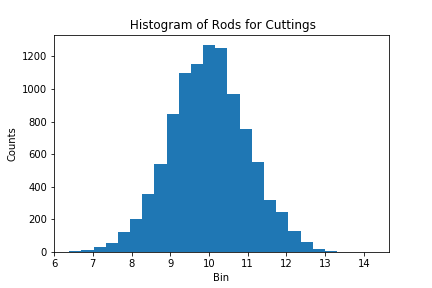
\includegraphics[width=1\linewidth,height=0.25\textheight]{Fig01}
\caption{1. Histogram Rods Variation}
\label{fig:Fig01}
\end{figure}

\noindent Question: \\ Given the specification of $\pm 1$, how many are good and what is the    yield? \\ 
\noindent Answer number of good rods = 6954, yield = 69.54\%. Note that everytime the program is run these    values changes. The solution was an algorithm to check dimension of each    rod and count those that are within tolerance. Solving it using (4) gives    a unique answer unlike the results from the algorithm above. Why?   \subsection{Equipment}    Now consider that these rods are to be cut into    halves. The cutter has $\mu = 0.5 $ and $\sigma = 0.1 $ then for 6954 pieces we have 
\begin{equation}
\begin{minipage}{300pt}
 $\displaystyle f_{1} = NormalDistribution(0.5, 0.1)$  
\end{minipage}
\end{equation}
\begin{equation}
\begin{minipage}{300pt}
 $\displaystyle f{_1}(z) = \frac{5.0 \sqrt{2} e^{- 50.0 \left(z - 0.5\right)^{2}}}{\sqrt{\pi}}$  
\end{minipage}
\end{equation}
\begin{equation}
\begin{minipage}{300pt}
 $\displaystyle f{_2}(z) = \int_{z_{i}}^{z_{f}} f{_1}(z)\, dz$  
\end{minipage}
\end{equation}
\begin{equation}
\begin{minipage}{300pt}
 $\displaystyle Cut_{event} = random.normal(0.5, 0.1, 6954) =  \newline  [0.5104791588224948, 0.5032845297161098, \dots \\ 0.4233040541115318] $  
\end{minipage}
\end{equation}
\noindent The histogram of (19) is shown in Figure 2.
\begin{figure}[H]
\centering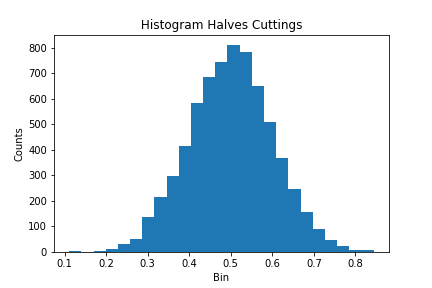
\includegraphics[width=1\linewidth,height=0.25\textheight]{Fig02}
\caption{Histogram of Cutter Variation}
\label{fig:Fig02}
\end{figure}

\noindent \subsection{Method}    There two methods to cut the rod. One method is the cutter is place at  a    distance of half the rod size exactly 5. Then the rod is referenced at the    point of origin and cut is made.  The other method is to place the rod    at its center for cutter engagement. The formulas for the two methods are    different. \\ \\ Question: Determine the formula for each and justify it.
\noindent \\ Answers: \\  1. The cutter with variation, i.e., $0.5 \pm .1$  is    multiplied by the perfect dimension of rod that is 10. Why perfect 10?    Then the answer is substracted from a rod with variation. The two answers    are the cut products.    \\ 2. The rod with variation, i.e., $ 10 \pm 1$ is multiplied by the    cutter with variation, i.e., $0.5 \pm .1$. The answer is substracted from    the rod with variation. The two cuts are products. \\ 
\noindent The histograms of Method 1 and 2 are shown in Figure 3.
\begin{figure}[H]
\centering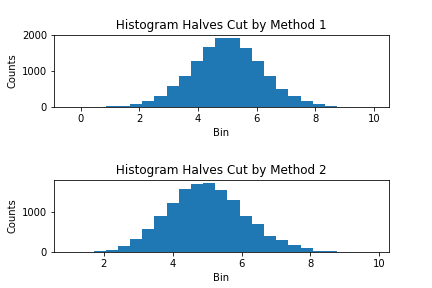
\includegraphics[width=1\linewidth,height=0.25\textheight]{Fig03}
\caption{Histogram of Cut Rods}
\label{fig:Fig03}
\end{figure}

\noindent Question: \\ Assuming that the cut specification is $5 \pm .5$, determine the number    of good cut and the yield for each method \\ 
\noindent Answer: \\ 1. The number of good cut for method 1 is $4557 $ while for method 2 $4780 $ respectively. \\ 
\noindent 2. The yield for method 1 is $32.7653 $\% while for method 2 is $34.3687 $\% respectively. Why is it method 2 has higher yield? \\ \\    \subsection{Operator}    Assume and operator makes the loading with error of $\mu = 0.4 $ and $\sigma = 0.1 $. 
\noindent The histograms with operator handling for Method 1 and 2 are shown in     Figure 4.
\begin{figure}[H]
\centering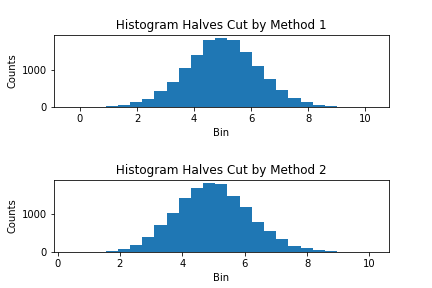
\includegraphics[width=1\linewidth,height=0.25\textheight]{Fig04}
\caption{Histogram of Cut Rods with    Operator's Handling}
\label{fig:Fig04}
\end{figure}

\noindent The yield with operator's handling errors for method 1 is $31 $\% while for method 2 is $32 $\% respectively.
\noindent \section{Discussion}\subsection{Tolerance Variation}The yield numbers were exagerated for theoretical discussion. The four    variables are material, equipment or machine, method, and operator or man.    Hences, such sources of variations are known as 4M. \\ \\    In real world, the overall yied is the only one observed and reported. It    problematict to account the yield loss for each source. However, the so-called    fool proofing refers to elimination of operator's mishandling. Tyically the    solution is jig and fixture. In this case, the positional fixture with    alignment jig could eliminate the operator's error. \\ \\    The variation in machine could increase overtime. Hence, regular caligration    is necessary. To improve the variability, the continuous improvement    probram is the typical solution. \\ \\    The material variation can be mitigated at a cost by simple requirement f0r    tighter tolerances. However, the most difficult variation to estimate is    the method. The difficulty was chosing the appropriate equation to define    the variability in a method. For instance, either of the two methods has    rejects of oversize.  It is possible to introduct rework or reprocess to    cut the oversize for yield recovery purposes. What are the appropriate    equations and the corresponding algorithm that can be concocted for each    method? If the target reference remains the mean, there is a chance that the    outcome is undersize. Should it the reference be at maximum tolerance?    In other words, the method for rework may not be the same as the standard    process. \subsection{Other Type of Variations}
\begin{figure}[H]
\centering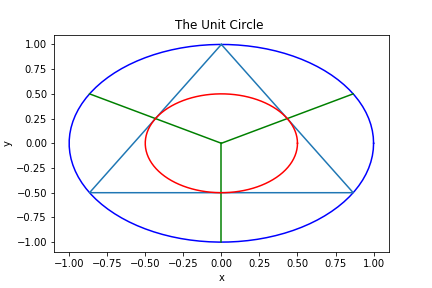
\includegraphics[width=1\linewidth,height=0.3\textheight]{Fig05}
\caption{Equilateral Triangle Inscribe in     Unit Circle}
\label{fig:Fig05}
\end{figure}

\noindent Consider a unit circle where an equilateral triangle is inscribed as    shown in Figure 5. Suppose a random line is to be drawn across it,    determine the probability that the cord is less than the length of the    the side of equilateral triangle. There are a number of answer depending    on how the random lines are drawn. \\    1. The line drawn from any two points at the circumference, gives the    probability of $\frac{1}{3}$. \\    2. The line drawn perpendicular to radius from a any point along radius gives the    probability of $\frac{1}{2}$ \\    3. The line drawn tangent to any concentric circle gives the probabiity    $\frac{1}{4}$. \\    4. From the length of the cord i.e. $0$ to $2$, the probability is    $\frac{\sqrt{3}}{2}$. \\ \\    The question is that which of the four probability numbers make sense? 
\noindent \section{Conclusion}The variation of process variables can simulated by pseudo random generator.     The formula or equation associated with the algorithm must be ensured     realistically. From theoretical perspective the variance of every variable     can be determined but in real world operation, the net variance is the     only one that can be measured. Hence, the defect modes may be difficult     to itemize. \\ \\     As discussed, the application of random variable depends on certain     perspective of variation. For instance, a short cord drawn near the center     of the circuit is not a line crossing the circle although it is random.     It hsd to be moved from the center to have its end points touch the     circumference. \\ \\     Finally, the accuracy must be the difference between the average and the     specified mean must be approaching zero. The precission or repeatability     must be such that the tolerance is equal to a number of sixmas. 
\noindent \section{Recommendation}The Monte Carlo Simulation is useful for prediction of process yield.     Due care should be excercised in formulation of equation and algorthm.     The mathematics must be articulate the real world. There exists ample     room for creativity in defect modes itemization. The design of experiments     were used to optimize parameters. The Monte Carlo Simulation may help     to reduce number of experiments.
\noindent \bibliographystyle{plain} 
 \bibliography{MCIEEE}
\noindent \section*{About the Authors}
\noindent \begin{IEEEbiography}[{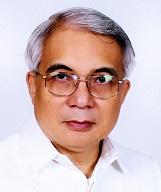
\includegraphics[width=.75in,height=1in,clip,               keepaspectratio]{cco.png}}]{Celso Bation Co} He earned his diploma as Electronic Technician from International        Correspondence Schools of University of Pennsylvania in 1972. He obtained        his degree of Bachelor of Science in Electronics and Communication        Engineering (ECE) from the University of Sto Tomas in 1977, Master         and Doctoral degrees in ECE from De La Salle University in 1996 and        2007 respectively. \\ He is currently the research director of Technological Institute of the        Philippines and an advocate of strong linkages among academes, industries        and government institutions.\end{IEEEbiography}\ \ \newline

\end{document}